\chapter{四旋翼无人机飞控建模}\label{le}
在本章,本文分三部分介绍四旋翼的飞控建模过程,\ref{1}节是飞行摇杆的数据传入过程,作为四旋翼无人机的姿态角的输入;\ref{2}节 是四旋翼无人机飞行动力学部分,也是本章的核心部分;\ref{3}节是三维视景系统的设计原理。关系如图\ref{fig17}所示。
\vspace{-10pt}
\begin{figure}[!ht]
\centering
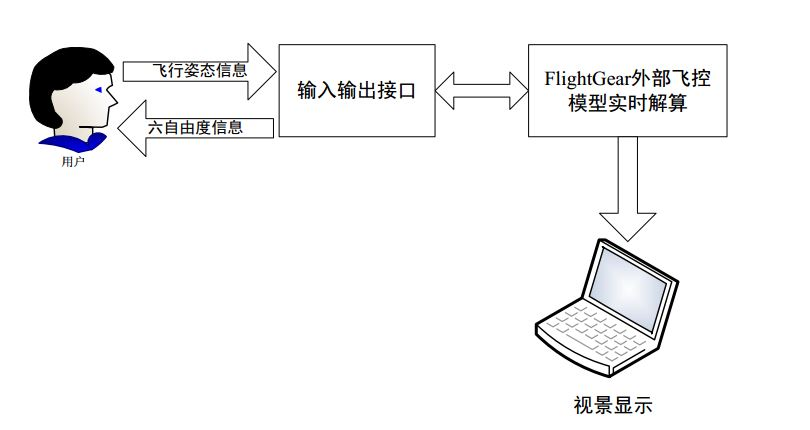
\includegraphics[width=0.8\textwidth]{f18.jpg}
\caption{四旋翼飞控建模过程}
\label{fig17}
\end{figure}
\vspace{-10pt}
\section{飞行摇杆数据传入}\label{1}
  本文将飞行摇杆(Joystick)数据读取作为四旋翼飞控模型的输入,Joystick数据的数据主要是四旋翼的姿态角(滚转角,偏航角,俯仰角)和四旋翼的推力。因此,本文通过C++编程,实现飞行摇杆数据的输入。由如下代码所示:

 \begin{lstlisting}[language={[ANSI]C++}]
class HAL_JoyStick: public ZY::Thread {
public:
    HAL_JoyStick(){
        m_devID = -1;
    }
    HAL_JoyStick(int dev) {
        m_devID=dev;
    }
    virtual ~HAL_JoyStick() {}
    int open(int devID);
    void run();
    int close(void);
    int read(JS_Val *jsv)
    {
        data_mutex.lock();
        *jsv= m_JSVal;
        m_JSVal.dataUpdated = 0;
        data_mutex.unlock();
        return 0;
    }
public:
    int         m_devType;
    int         m_devID;
    int         m_devFD;
    char        number_of_axes;
    char        number_of_btns;
protected:
    ZY::Mutex   data_mutex;
    JS_Val      m_JSVal;
}
\end{lstlisting}

\section{四旋翼飞控建模\ucite{4}}\label{2}
在本节中,分为三部分进行四旋翼飞行动力学建模的过程,第一部分是四旋翼飞行建模中需要的变量与坐标系的说明与定义;第二部分是推导六自由度四旋翼飞行动力学方程;第三部分是对模型进行化简,进行模型的求解。
  \subsection{四旋翼变量}
\begin{table}[!h]
\begin{center}
\caption{四旋翼参数表}\label{t1}
\begin{longtable}{ | c| c|}
\hline
参数名称                                    & 参数意义                                                                  \\\hline
${p_n}$                    & 惯性坐标系$\mathop R\nolimits^i $下,四旋翼$x$轴方向的位置                               \\\hline
${p_e}$           & 惯性坐标系$\mathop R\nolimits^i $下,四旋翼$y$轴方向的位置                                    \\\hline
$h$              & 惯性坐标系$\mathop R\nolimits^i $下, 四旋翼$z$轴方向的高度                                            \\\hline
$u$                      & 机体坐标系$\mathop R\nolimits^b $下,四旋翼$x$轴方向的速度
                                          \\\hline
$v$                 & 机体坐标系$\mathop R\nolimits^b $下,四旋翼$y$轴方向的速度
                          \\\hline
$\omega $ &  机体坐标系$\mathop R\nolimits^b $下,四旋翼$z$轴方向的速度
 \\\hline
$\phi $             & 滚转角
\\\hline
$\theta $ &俯仰角
\\\hline
$\psi $  &  偏航角
\\\hline
$p$ &   机体坐标系$\mathop R\nolimits^b $下,滚转角速率
\\\hline
$q$ &  机体坐标系$\mathop R\nolimits^b $下,俯仰角速率
\\\hline
$r$ &    机体坐标系$\mathop R\nolimits^b $下,偏航角速率
\\\hline
\end{longtable}
\end{center}
\end{table}
\vspace{-20pt}
如表\ref{t1}所示,四旋翼建模过程中所需的参数变量,将上述变量关系在图\ref{fig19}中所示。四旋翼姿态位置变量$\left( {{p_n},{p_e},h} \right)$是定义在惯性坐标系(即地面坐标系)下,其中,高度变量$h$在惯性坐标系下沿着$z$轴的负半轴方向,即方向向上。在机体坐标系下,定义四旋翼的速度变量$\left( {u,v,\omega } \right)$和角速度变量$\left( {p,q,r} \right)$。欧拉角(滚转角$\phi $,俯仰角$\theta $,$\psi $)分别定义与上章的滚转坐标系,俯仰坐标系和偏航坐标系下。

\begin{figure}[!ht]
\centering
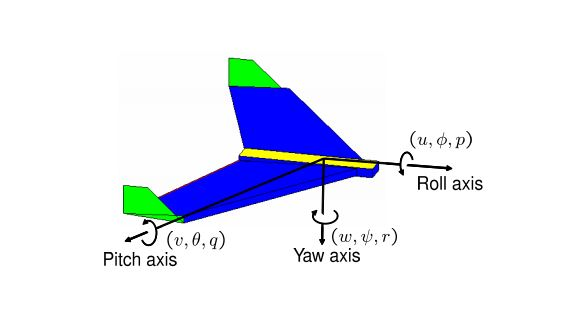
\includegraphics[width=0.7\textwidth]{f19.jpg}
\caption{坐标轴定义}
\label{fig19}
\end{figure}

  \subsection{四旋翼六自由度飞行动力学建模}
  \subsubsection{四旋翼运动学方程}
	在地面坐标系下,定义四旋翼姿态位置变量$\left( {{p_n},{p_e},h} \right)$;在机体坐标系下,定义四旋翼速度变量$\left( {u,v,\omega } \right)$。因此,需要建立位置变量与姿态变量之间的关系,结合2.1节坐标系转换的公式可得:

\[\begin{array}{l}
\frac{d}{{dt}}\left( \begin{array}{l}
{p_n}\\
{p_e}\\
 - h
\end{array} \right) = \mathop F\nolimits_b^v \left( \begin{array}{l}
u\\
v\\
\omega
\end{array} \right)\\
{\kern 1pt} {\kern 1pt} {\kern 1pt} {\kern 1pt} {\kern 1pt} {\kern 1pt} {\kern 1pt} {\kern 1pt} {\kern 1pt} {\kern 1pt} {\kern 1pt} {\kern 1pt} {\kern 1pt} {\kern 1pt} {\kern 1pt} {\kern 1pt} {\kern 1pt} {\kern 1pt} {\kern 1pt} {\kern 1pt} {\kern 1pt} {\kern 1pt} {\kern 1pt} {\kern 1pt} {\kern 1pt} {\kern 1pt} {\kern 1pt} {\kern 1pt} {\kern 1pt} {\kern 1pt} {\kern 1pt} {\kern 1pt} {\kern 1pt} {\kern 1pt} {\kern 1pt} {\kern 1pt} {\kern 1pt} {\kern 1pt} {\kern 1pt} {\kern 1pt} {\kern 1pt} {\kern 1pt} {\kern 1pt} {\kern 1pt} {\kern 1pt} {\kern 1pt} {\kern 1pt} {\kern 1pt} {\kern 1pt} {\kern 1pt} {\kern 1pt} {\kern 1pt} {\kern 1pt} {\kern 1pt} {\kern 1pt} {\kern 1pt} {\kern 1pt} {\kern 1pt} {\kern 1pt}  = {\left( {\mathop F\nolimits_b^v } \right)^T}\left( \begin{array}{l}
u\\
v\\
\omega
\end{array} \right)\\
{\kern 1pt} {\kern 1pt} {\kern 1pt} {\kern 1pt} {\kern 1pt} {\kern 1pt} {\kern 1pt} {\kern 1pt} {\kern 1pt} {\kern 1pt} {\kern 1pt} {\kern 1pt} {\kern 1pt} {\kern 1pt} {\kern 1pt} {\kern 1pt} {\kern 1pt} {\kern 1pt} {\kern 1pt} {\kern 1pt} {\kern 1pt} {\kern 1pt} {\kern 1pt} {\kern 1pt} {\kern 1pt} {\kern 1pt} {\kern 1pt} {\kern 1pt} {\kern 1pt} {\kern 1pt} {\kern 1pt} {\kern 1pt} {\kern 1pt} {\kern 1pt} {\kern 1pt} {\kern 1pt} {\kern 1pt} {\kern 1pt} {\kern 1pt} {\kern 1pt} {\kern 1pt} {\kern 1pt} {\kern 1pt} {\kern 1pt} {\kern 1pt} {\kern 1pt} {\kern 1pt} {\kern 1pt} {\kern 1pt} {\kern 1pt} {\kern 1pt} {\kern 1pt} {\kern 1pt} {\kern 1pt} {\kern 1pt} {\kern 1pt} {\kern 1pt}  = \left( {\begin{array}{*{20}{c}}
{c\theta c\psi }&{s\phi s\theta c\psi  - c\phi s\psi }&{c\phi s\theta c\psi  + s\theta s\psi }\\
{c\theta s\psi }&{s\phi s\theta s\psi  + c\phi c\psi }&{c\phi s\theta s\psi  - s\theta c\psi }\\
{ - s\theta }&{s\phi c\theta }&{c\phi c\theta }
\end{array}} \right)\left( \begin{array}{l}
u\\
v\\
\omega
\end{array} \right)
\end{array}\]

其中,$c = \cos {\kern 1pt} ,s = \sin $。

同样,欧拉角(滚转角$\phi $,俯仰角$\theta $,$\psi $)和角速度$\left( {p,q,r} \right)$之间也需要坐标系的转换。但是,它们之间坐标系的转换是复杂的,角速度变量被定义于机体坐标系,但是,欧拉角分别定义于三个不同的坐标系,即滚转角坐标系,俯仰角坐标系和偏航角坐标系(2.1节所示)。于是,我们需要建立起角速度$\left( {p,q,r} \right)$和欧拉角速率$\left( {\mathop \phi \limits^ \cdot  ,\mathop \theta \limits^ \cdot  ,\mathop \psi \limits^ \cdot  } \right)$之间的关系。因为欧拉角速率均为小量,可以近似于欧拉角与角速度之间的关系。
\[\mathop F\nolimits_{v2}^b \left( {\mathop \phi \limits^ \cdot  } \right) = \mathop F\nolimits_{v1}^{v2} \left( {\mathop \theta \limits^ \cdot  } \right) = \mathop F\nolimits_v^{v1} \left( {\mathop \psi \limits^ \cdot  } \right)\]
因此,我们可以得到:
\small
\begin{equation}
\begin{array}{l}
\left( \begin{array}{l}
p\\
q\\
r
\end{array} \right) = \mathop R\nolimits_{v2}^b \left( {\mathop \phi \limits^ \cdot  } \right)\left( \begin{array}{l}
\mathop \phi \limits^ \cdot  \\
0\\
0
\end{array} \right) + \mathop R\nolimits_{v2}^b \left( \phi  \right)\mathop R\nolimits_{v1}^{v2} \left( {\mathop \theta \limits^ \cdot  } \right)\left( \begin{array}{l}
0\\
\mathop \theta \limits^ \cdot  \\
0
\end{array} \right) + \mathop R\nolimits_{v2}^b \left( \phi  \right)\mathop R\nolimits_{v1}^{v2} \left( {\mathop \theta \limits^ \cdot  } \right)\mathop R\nolimits_{v \to v1} \left( {\mathop \psi \limits^ \cdot  } \right)\left( \begin{array}{l}
0\\
0\\
\mathop \psi \limits^ \cdot
\end{array} \right)\\
{\kern 1pt}  = \left( \begin{array}{l}
\mathop \phi \limits^ \cdot  \\
0\\
0
\end{array} \right) + \left( {\begin{array}{*{20}{c}}
1&0&0\\
0&{\cos \phi }&{\sin \phi }\\
0&{ - \sin \phi }&{\cos \phi }
\end{array}} \right)\left( \begin{array}{l}
0\\
\mathop \theta \limits^ \cdot  \\
0
\end{array} \right) + \left( {\begin{array}{*{20}{c}}
1&0&0\\
0&{\cos \phi }&{\sin \phi }\\
0&{ - \sin \phi }&{\cos \phi }
\end{array}} \right)\left( {\begin{array}{*{20}{c}}
{\cos \theta }&0&{ - \sin \theta }\\
0&1&0\\
{\sin \theta }&0&{\cos \theta }
\end{array}} \right)\\
 = \left( {\begin{array}{*{20}{c}}
1&0&{ - s\theta }\\
0&{{\mathop{\rm c}\nolimits} \phi }&{{\mathop{\rm s}\nolimits} \phi c\theta }\\
0&{ - {\mathop{\rm s}\nolimits} \phi }&{c\phi c\theta }
\end{array}} \right)\left( \begin{array}{l}
\mathop \phi \limits^ \cdot  \\
\mathop \theta \limits^ \cdot  \\
\mathop \psi \limits^ \cdot
\end{array} \right)
\end{array}
\end{equation}
\small
通过,对上式求逆可得:
\begin{equation}
\left( \begin{array}{l}
\mathop \phi \limits^ \cdot  \\
\mathop \theta \limits^ \cdot  \\
\mathop \psi \limits^ \cdot
\end{array} \right) = \left( {\begin{array}{*{20}{c}}
1&{\sin \left( \phi  \right)\tan \left( \theta  \right)}&{\cos \left( \phi  \right)\tan \left( \theta  \right)}\\
0&{\cos \left( \phi  \right)}&{ - \sin \left( \phi  \right)}\\
0&{\sin \left( \phi  \right)\sec \left( \theta  \right)}&{\cos \left( \phi  \right)\sec \left( \theta  \right)}
\end{array}} \right)\left( \begin{array}{l}
p\\
q\\
r
\end{array} \right)
\end{equation}

在惯性坐标系下,根据牛顿第二定律的微分形式,可以得到四旋翼的速度与力之间的关系,如下所示:
\[m\frac{{d{\bf{v}}}}{{d{t_i}}} = {\bf{f}}\]

其中,$m$是四旋翼的质量,${\bf{f}}$是四旋翼的合力,$\frac{d}{{d{t_i}}}$是四旋翼在惯性坐标系下的时间导数。根据2.1.3节的Coriolis公式可得:
\begin{equation}
m\frac{{d{\bf{v}}}}{{d{t_i}}} = m\left( {\frac{{d{\bf{v}}}}{{d{t_b}}} + {\omega _{b/i}} \times {\bf{v}}} \right) = {\bf{f}}
\end{equation}

其中,${\omega _{b/i}}$是在惯性坐标系下的角速度,因为四旋翼的受力是在机体坐标系下计算的,所以,$\omega$在机体坐标系下进行测量,利用上式,结合${{\bf{v}}^b} \buildrel \Delta \over = {\left( {u,v,\omega } \right)^T}$和${\omega _{b/i}} \buildrel \Delta \over = {\left( {p,q,r} \right)^T}$关系式以及${{\bf{f}}^b} \buildrel \Delta \over = {\left( {{f_x},{f_y},{f_z}} \right)^T}$上式可以表示为:
\begin{equation}
\left( \begin{array}{l}
\mathop u\limits^ \cdot  \\
\mathop \nu \limits^ \cdot  \\
\mathop \omega \limits^ \cdot
\end{array} \right) = \left( \begin{array}{l}
rv - q\omega \\
p\omega  - ru\\
qu - pv
\end{array} \right) + \frac{1}{m}\left( \begin{array}{l}
{f_x}\\
{f_y}\\
{f_z}
\end{array} \right)
\end{equation}

对于旋转运动而言,由牛顿第二定律可得:
\begin{equation}
\frac{{d{{\bf{h}}^b}}}{{d{t_i}}} = m
\end{equation}

其中,$h$代表角动量,$m$是力矩,利用Coriolis公式可得:
\[\frac{{d{\bf{h}}}}{{d{t_i}}} = \frac{{d{\bf{h}}}}{{d{t_b}}} + {\omega _{b/i}} \times {\bf{h}} = {\bf{m}}\]

将上式在机体坐标系下,进行求解,其中,${{\bf{h}}^b} = {\bf{J}}\omega _{b/i}^i$,${\bf{J}}$是常量的惯性矩阵。
\[\begin{array}{l}
{\bf{J}} = \left( {\begin{array}{*{20}{c}}
{\int {\left( {{y^2} + {z^2}} \right)dm} }&{ - \int {xydm} }&{ - \int {xzdm} }\\
{ - \int {xydm} }&{\int {\left( {{x^2} + {z^2}} \right)dm} }&{ - \int {yzdm} }\\
{ - \int {xzdm} }&{ - \int {yzdm} }&{\int {\left( {{x^2} + {y^2}} \right)dm} }
\end{array}} \right)\\
{\kern 1pt} {\kern 1pt} {\kern 1pt} {\kern 1pt} {\kern 1pt} {\kern 1pt} {\kern 1pt} {\kern 1pt} {\kern 1pt} {\kern 1pt} {\kern 1pt} {\kern 1pt} {\kern 1pt}  \buildrel \Delta \over = \left( {\begin{array}{*{20}{c}}
{{J_x}}&{ - {J_{xy}}}&{ - {J_{xz}}}\\
{ - {J_{xy}}}&{{J_y}}&{ - {J_{yz}}}\\
{ - {J_{xz}}}&{ - {J_{yz}}}&{{J_z}}
\end{array}} \right)
\end{array}\]
\vspace{-10pt}
\begin{figure}[!ht]
\centering
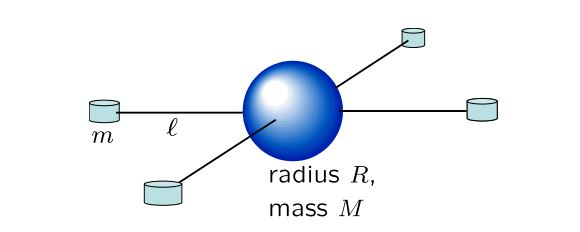
\includegraphics[width=0.7\textwidth]{f12.jpg}
\caption{四旋翼力矩图\ucite{4}}
\label{fig20}
\end{figure}
如图\ref{fig20}所示,四旋翼关于三个坐标轴几何对称性,因此${J_{xy}} = {J_{xz}} = {J_{yz}} = 0$,可得
\[J = \left( {\begin{array}{*{20}{c}}
{{J_x}}&0&0\\
0&{{J_y}}&0\\
0&0&{{J_z}}
\end{array}} \right)\]

因此,
\[{J^{ - 1}} = \left( {\begin{array}{*{20}{c}}
{\frac{1}{{{J_x}}}}&0&0\\
0&{\frac{1}{{{J_y}}}}&0\\
0&0&{\frac{1}{{{J_z}}}}
\end{array}} \right)\]

如图\ref{fig20}所示,球体的转动惯量为$J = \frac{2}{5}M{R^2}$,从而就可得到:
\[\begin{array}{l}
{J_x} = \frac{2}{5}M{R^2} + 2{l^2}m\\
{J_y} = \frac{2}{5}M{R^2} + 2{l^2}m\\
{J_z} = \frac{2}{5}M{R^2} + 4{l^2}m
\end{array}\]

定义力矩${m^b} \buildrel \Delta \over = {\left( {{\tau _\phi },{\tau _\theta },{\tau _\psi }} \right)^T}$,代入公式
(3.5)可得:
\[\begin{array}{l}
\left( \begin{array}{l}
\mathop p\limits^ \cdot  \\
\mathop q\limits^ \cdot  \\
\mathop r\limits^ \cdot
\end{array} \right) = \left( {\begin{array}{*{20}{c}}
{\frac{1}{{{J_x}}}}&0&0\\
0&{\frac{1}{{{J_y}}}}&0\\
0&0&{\frac{1}{{{J_z}}}}
\end{array}} \right)\left[ {\left( {\begin{array}{*{20}{c}}
0&r&{ - q}\\
{ - r}&0&p\\
q&{ - p}&0
\end{array}} \right)\left( {\begin{array}{*{20}{c}}
{{J_x}}&0&0\\
0&{{J_y}}&0\\
0&0&{{J_z}}
\end{array}} \right)\left( \begin{array}{l}
p\\
q\\
r
\end{array} \right) + \left( \begin{array}{l}
{\tau _\phi }\\
{\tau _\theta }\\
{\tau _\psi }
\end{array} \right)} \right]\\
{\kern 1pt} {\kern 1pt} {\kern 1pt} {\kern 1pt} {\kern 1pt} {\kern 1pt} {\kern 1pt} {\kern 1pt} {\kern 1pt} {\kern 1pt} {\kern 1pt} {\kern 1pt} {\kern 1pt} {\kern 1pt} {\kern 1pt} {\kern 1pt} {\kern 1pt} {\kern 1pt}  = \left( \begin{array}{l}
\frac{{{J_y} - {J_z}}}{{{J_x}}}qr\\
\frac{{{J_z} - {J_x}}}{{{J_y}}}pr\\
\frac{{{J_x} - {J_y}}}{{{J_z}}}pq
\end{array} \right) + \left( \begin{array}{l}
\frac{1}{{{J_x}}}{\tau _\phi }\\
\frac{1}{{{J_y}}}{\tau _\theta }\\
\frac{1}{{{J_z}}}{\tau _\psi }
\end{array} \right)\\
{\kern 1pt} {\kern 1pt} {\kern 1pt} {\kern 1pt} {\kern 1pt} {\kern 1pt} {\kern 1pt}
\end{array}\]

最后,六自由度飞行动力学方程如下所示。
\begin{equation}
\left( \begin{array}{c}
\mathop {{p_n}}\limits^ \cdot  \\
\mathop {{p_e}}\limits^ \cdot  \\
h
\end{array} \right) = \left( {\begin{array}{*{20}{c}}
{c\theta c\psi }&{s\phi s\theta c\psi  - c\phi s\psi }&{c\phi s\theta c\psi  + s\phi s\psi }\\
{c\theta s\psi }&{s\phi s\theta s\psi  + c\phi c\psi }&{c\phi s\theta s\psi  - s\phi c\psi }\\
{s\theta }&{ - s\phi c\theta }&{ - c\phi c\theta }
\end{array}} \right)\left( \begin{array}{l}
u\\
v\\
\omega
\end{array} \right)
\end{equation}
\begin{equation}
\left( \begin{array}{l}
\mathop u\limits^ \cdot  \\
\mathop v\limits^ \cdot  \\
\mathop \omega \limits^ \cdot
\end{array} \right) = \left( \begin{array}{l}
rv - q\omega \\
p\omega  - ru\\
qu - pv
\end{array} \right) + \frac{1}{m}\left( \begin{array}{l}
{f_x}\\
{f_y}\\
{f_z}
\end{array} \right)
\end{equation}
\begin{equation}
\left( \begin{array}{l}
\mathop \phi \limits^ \cdot  \\
\mathop \theta \limits^ \cdot  \\
\mathop \psi \limits^ \cdot
\end{array} \right) = \left( {\begin{array}{*{20}{c}}
1&{\sin \phi \tan \theta }&{\cos \phi \tan \theta }\\
0&{\cos \phi }&{ - \sin \phi }\\
0&{\frac{{\sin \phi }}{{\cos \theta }}}&{\frac{{\cos \phi }}{{\cos \theta }}}
\end{array}} \right)\left( \begin{array}{l}
p\\
q\\
r
\end{array} \right)
\end{equation}
\begin{equation}
\left( \begin{array}{l}
\mathop p\limits^ \cdot  \\
\mathop q\limits^ \cdot  \\
\mathop r\limits^ \cdot
\end{array} \right) = \left( \begin{array}{l}
\frac{{{J_y} - {J_z}}}{{{J_x}}}qr\\
\frac{{{J_z} - {J_x}}}{{{J_y}}}pr\\
\frac{{{J_x} - {J_y}}}{{{J_z}}}pq
\end{array} \right) + \left( \begin{array}{l}
\frac{1}{{{J_x}}}{\tau _\phi }\\
\frac{1}{{{J_y}}}{\tau _\theta }\\
\frac{1}{{{J_z}}}{\tau _\psi }
\end{array} \right)
\end{equation}

\subsubsection{四旋翼力和力矩方程}
对于四旋翼而言,因为没有空气动力学的升力面,所以,四旋翼的气动力和气动力矩是可以忽略的。四旋翼的力和力矩主要来自于重力和四个螺旋桨的推力。如图\ref{fig21}所示。
\vspace{-20pt}
\begin{figure}[!ht]
\centering
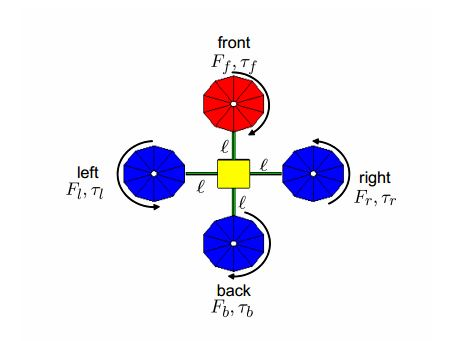
\includegraphics[width=0.7\textwidth]{f13.jpg}
\caption{四旋翼力和力矩俯视图\ucite{4}}
\label{fig21}
\end{figure}

\begin{figure}[!ht]
\centering
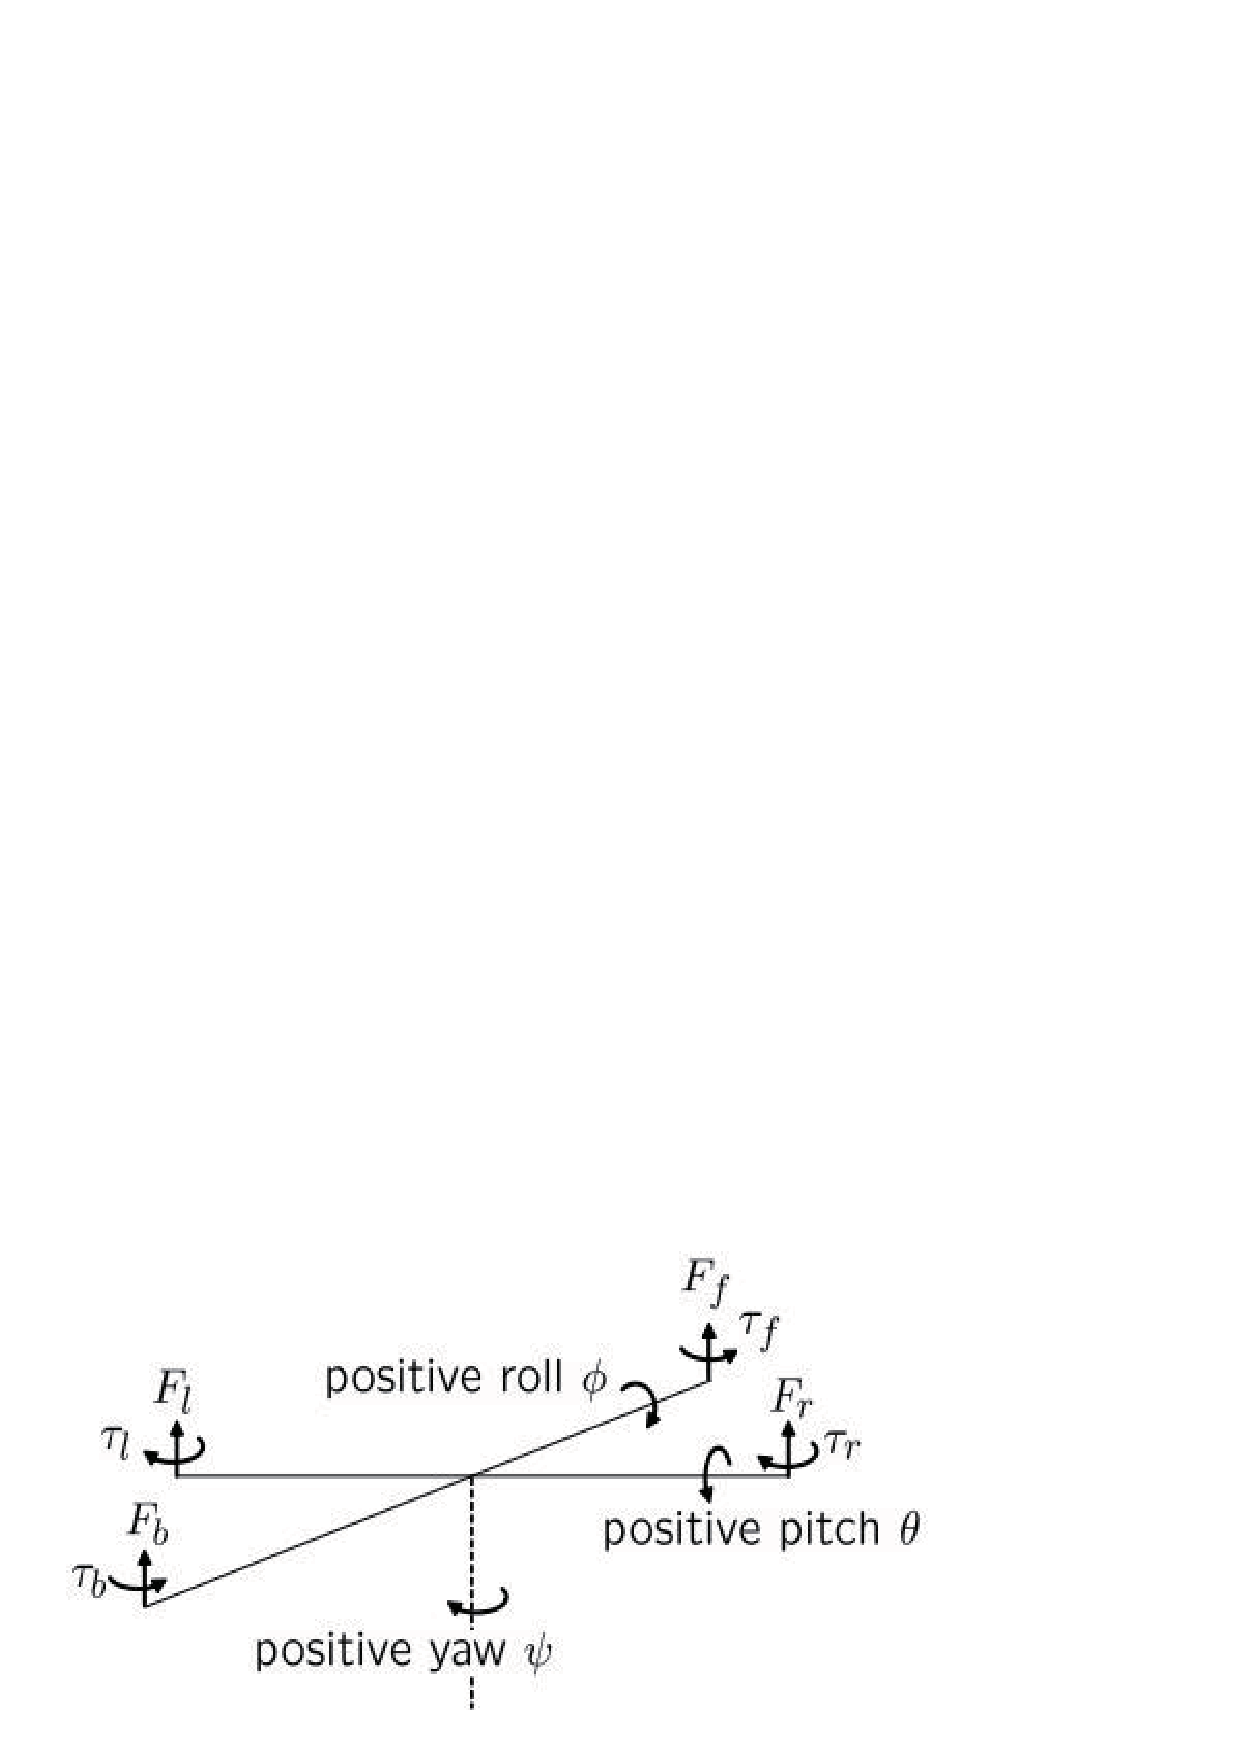
\includegraphics[width=0.7\textwidth]{f14.jpg}
\caption{四旋翼力和力矩俯视图\ucite{4}}
\label{fig22}
\end{figure}
由图\ref{fig21}所示,是从四旋翼的俯视图来得到的力和力矩图。图\ref{fig22}所示的四旋翼力和力矩的受力简化图,每个螺旋剑电机产生力和力矩。作用于四旋翼上的力可以表示为:
\[F = {F_f} + {F_r} + {F_b} + {F_l}\]

如图\ref{fig22}所示,左右电机产生的滚转力矩可以表示为:
\[{\tau _\phi } = l\left( {{F_l} - {F_r}} \right)\]

同理,前后电机产生的俯仰力矩可以表示为:
\[{\tau _\theta } = l\left( {{F_f} - {F_b}} \right)\]

由牛顿第三定律可知,阻力产生的偏航力矩反作用于四旋翼,方向与四旋翼的旋转方向相反。因此,四旋翼的旋转矩阵可以表示为:
\[{\tau _\psi } = {\tau _r} + {\tau _l} - {\tau _f} - {\tau _b}\]

由螺旋桨产生的升力和阻力,与角速度的平方成线性关系,如下所示:
\[\begin{array}{l}
{F_ * }{\rm{  = }}{k_1}{\delta _ * }\\
{\tau _ * } = {k_2}{\delta _ * }
\end{array}\]

其中,系数${k_1}$和${k_2}$由实验可以测得,${\delta _ * }$电机控制的信号,$ * $表示$f$,$r$,$b$,$l$电机。作用在四旋翼上力和力矩的矩阵如下所示:
\[\left( \begin{array}{l}
F\\
{\tau _\phi }\\
{\tau _\theta }\\
{\tau _\psi }
\end{array} \right) = \left( {\begin{array}{*{20}{c}}
{{k_1}}&{{k_1}}&{{k_1}}&{{k_1}}\\
0&{ - l{k_1}}&0&{l{k_1}}\\
{l{k_1}}&0&{l{k_1}}&0\\
{ - {k_2}}&{{k_2}}&{ - {k_2}}&{{k_2}}
\end{array}} \right)\left( \begin{array}{l}
{\delta _f}\\
{\delta _r}\\
{\delta _b}\\
{\delta _l}
\end{array} \right) \buildrel \Delta \over = M\left( \begin{array}{l}
{\delta _f}\\
{\delta _r}\\
{\delta _b}\\
{\delta _l}
\end{array} \right)\]

四旋翼除了受电机产生的作用力外,还有自身的重力,在速度坐标系$\mathop R\nolimits^v $下,重力恰好作用与坐标系的重心位置,故:
\[\mathop f\nolimits_g^v  = \left( \begin{array}{c}
0\\
0\\
mg
\end{array} \right)\]

但是,速度是在机体坐标系下表示的,故上式需转换在机体坐标系下:
\[\begin{array}{l}
\mathop f\nolimits_g^b  = \mathop R\nolimits_v^b \left( \begin{array}{c}
0\\
0\\
mg
\end{array} \right)\\
{\kern 1pt} {\kern 1pt} {\kern 1pt} {\kern 1pt} {\kern 1pt} {\kern 1pt} {\kern 1pt} {\kern 1pt} {\kern 1pt} {\kern 1pt} {\kern 1pt} {\kern 1pt} {\kern 1pt} {\kern 1pt} {\kern 1pt} {\kern 1pt} {\kern 1pt} {\kern 1pt} {\kern 1pt}  = \left( \begin{array}{l}
 - mg\sin \theta \\
mg\cos \theta \sin \phi \\
mg\cos \theta \cos \phi
\end{array} \right)
\end{array}\]

最终,四旋翼的六自由度飞行动力学模型如下:
\begin{equation}
\left( \begin{array}{c}
\mathop {{p_n}}\limits^ \cdot  \\
\mathop {{p_e}}\limits^ \cdot  \\
h
\end{array} \right) = \left( {\begin{array}{*{20}{c}}
{c\theta c\psi }&{s\phi s\theta c\psi  - c\phi s\psi }&{c\phi s\theta c\psi  + s\phi s\psi }\\
{c\theta s\psi }&{s\phi s\theta s\psi  + c\phi c\psi }&{c\phi s\theta s\psi  - s\phi c\psi }\\
{s\theta }&{ - s\phi c\theta }&{ - c\phi c\theta }
\end{array}} \right)\left( \begin{array}{l}
u\\
v\\
\omega
\end{array} \right)
\end{equation}
\begin{equation}
\left( \begin{array}{l}
\mathop u\limits^ \cdot  \\
\mathop v\limits^ \cdot  \\
\mathop \omega \limits^ \cdot
\end{array} \right) = \left( \begin{array}{l}
rv - q\omega \\
p\omega  - ru\\
qu - pv
\end{array} \right) + \left( \begin{array}{c}
 - g\sin \theta \\
g\cos \theta \sin \phi \\
g\cos \theta \cos \phi
\end{array} \right) + \frac{1}{m}\left( \begin{array}{c}
0\\
0\\
 - F
\end{array} \right)
\end{equation}
\begin{equation}
\left( \begin{array}{l}
\mathop \phi \limits^ \cdot  \\
\mathop \theta \limits^ \cdot  \\
\mathop \psi \limits^ \cdot
\end{array} \right) = \left( {\begin{array}{*{20}{c}}
1&{\sin \phi \tan \theta }&{\cos \phi \tan \theta }\\
0&{\cos \phi }&{ - \sin \phi }\\
0&{\frac{{\sin \phi }}{{\cos \theta }}}&{\frac{{\cos \phi }}{{\cos \theta }}}
\end{array}} \right)\left( \begin{array}{l}
p\\
q\\
r
\end{array} \right)
\end{equation}
\begin{equation}
\left( \begin{array}{l}
\mathop p\limits^ \cdot  \\
\mathop q\limits^ \cdot  \\
\mathop r\limits^ \cdot
\end{array} \right) = \left( \begin{array}{l}
\frac{{{J_y} - {J_z}}}{{{J_x}}}qr\\
\frac{{{J_z} - {J_x}}}{{{J_y}}}pr\\
\frac{{{J_x} - {J_y}}}{{{J_z}}}pq
\end{array} \right) + \left( \begin{array}{l}
\frac{1}{{{J_x}}}{\tau _\phi }\\
\frac{1}{{{J_y}}}{\tau _\theta }\\
\frac{1}{{{J_z}}}{\tau _\psi }
\end{array} \right)
\end{equation}

\subsection{模型求解}

六自由度的四旋翼飞行动力学方程太复杂对于模型求解而言。本文基于小扰动假设,即果运动参数偏离基准状态的量为小量,可以略去二阶以上的运动参数变化量。在线性化的过程中,可以把无人机运动近似的分解为纵向运动和横向运动,两种运动相互独立。纵向运动即是飞机的俯仰运动;横向运动对应的是飞机的偏航与滚转运动。

假设$\phi$和$\theta$都是小量可以忽略,故公式(3.12)可以简化为:
\[\left( \begin{array}{l}
\mathop \phi \limits^ \cdot  \\
\mathop \theta \limits^ \cdot  \\
\mathop \psi \limits^ \cdot
\end{array} \right) = \left( \begin{array}{l}
p\\
q\\
r
\end{array} \right)\]

同理,假设Coriolis方程中$qr$,$pr$,$pq$均为小量可以忽略,故公式(3.13)可以简化为:
\[\left( \begin{array}{l}
\mathop p\limits^ \cdot  \\
\mathop q\limits^ \cdot  \\
\mathop r\limits^ \cdot
\end{array} \right) = \left( \begin{array}{l}
\frac{1}{{{J_x}}}{\tau _\phi }\\
\frac{1}{{{J_y}}}{\tau _\theta }\\
\frac{1}{{{J_z}}}{\tau _\psi }
\end{array} \right)\]

结合上面两式,可得:
\begin{equation}
\left( \begin{array}{l}
\mathop \phi \limits^{ \cdot  \cdot } \\
\mathop \theta \limits^{ \cdot  \cdot } \\
\mathop \psi \limits^{ \cdot  \cdot }
\end{array} \right) = \left( \begin{array}{l}
\frac{1}{{{J_x}}}{\tau _\phi }\\
\frac{1}{{{J_y}}}{\tau _\theta }\\
\frac{1}{{{J_z}}}{\tau _\psi }
\end{array} \right)
\end{equation}

对公式(3.10)求微分可得:
\[\left( {\begin{array}{*{20}{c}}
{c\theta c\psi }&{s\phi s\theta c\psi  - c\phi s\psi }&{c\phi s\theta c\psi  + s\phi c\psi }\\
{c\theta s\psi }&{s\phi s\theta s\psi  + c\phi c\psi }&{c\phi s\theta s\psi  - s\phi c\psi }\\
{ - s\theta }&{s\phi c\theta }&{c\phi c\theta }
\end{array}} \right)\]

对公式(3.11)忽略Coriolis量,代入上式可得:
\[\left( \begin{array}{l}
\mathop {{p_n}}\limits^{ \cdot  \cdot } \\
\mathop {{p_e}}\limits^{ \cdot  \cdot } \\
\mathop {{p_d}}\limits^{ \cdot  \cdot }
\end{array} \right) = \left( \begin{array}{l}
0\\
0\\
g
\end{array} \right) + \left( \begin{array}{c}
 - c\phi s\theta c\psi  - s\phi s\psi \\
 - c\phi s\theta s\psi  + s\phi c\psi \\
 - c\phi c\theta
\end{array} \right)\frac{F}{m}\]

因此,在惯性坐标系下,简化的方程如下:
\begin{equation}
\mathop {{p_n}}\limits^{ \cdot  \cdot }  = \left( { - \cos \phi \sin \theta \cos \psi  - \sin \phi \sin \psi } \right)\frac{F}{m}
\end{equation}
\begin{equation}
\mathop {{p_e}}\limits^{ \cdot  \cdot }  = \left( { - \cos \phi \sin \theta sin\psi  + \sin \phi \cos \psi } \right)\frac{F}{m}
\end{equation}
\begin{equation}
\mathop {{p_d}}\limits^{ \cdot  \cdot }  = g - \left( {\cos \phi \cos \theta } \right)\frac{F}{m}
\end{equation}
\begin{equation}
\mathop \phi \limits^{ \cdot  \cdot }  = \frac{1}{{{J_x}}}{\tau _\phi }
\end{equation}
\begin{equation}
\mathop \theta \limits^{ \cdot  \cdot }  = \frac{1}{{{J_y}}}{\tau _\theta }
\end{equation}
\begin{equation}
\mathop \psi \limits^{ \cdot  \cdot }  = \frac{1}{{{J_z}}}{\tau _\psi }
\end{equation}

\section{三维视景系统}\label{3}

三维可视仿真系统的结构如图 \ref{fig23}所示,主要包括仿真模块、飞行数据模块、通信模块、飞机模型库、纹理材质库等。
\vspace{-10pt}
\begin{figure}[!ht]
\centering
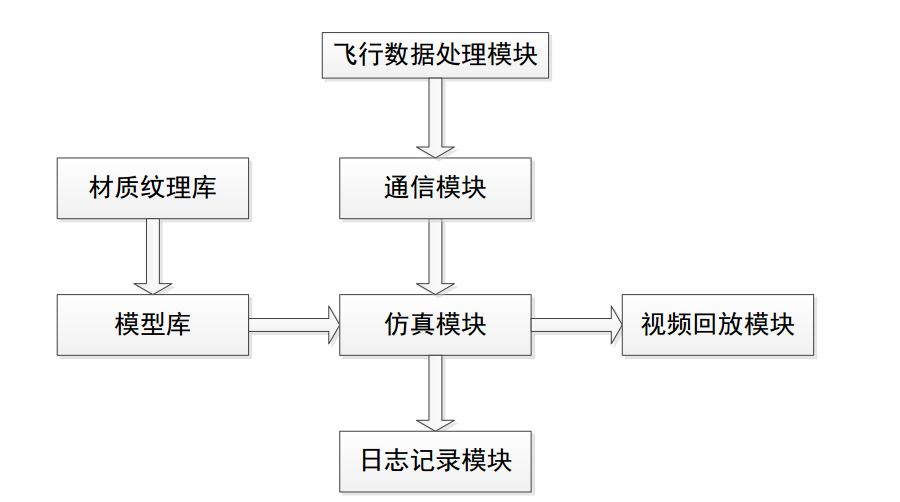
\includegraphics[width=0.7\textwidth]{f21.jpg}
\caption{三维可视化仿真结构图\ucite{16}}
\label{fig23}
\end{figure}

仿真模块是三维可视仿真系统的核心模块。一般使用高级程序语言(如 C++)编写,也可以调用第三方三维可视仿真软件实现。仿真模块主要完成以下功能\ucite{17}:
\begin{itemize}
  \item  接收通信模块传来的飞行数据。
  \item  从模型库中导入飞行器模型、场景模型、声音模型,并对飞行器进行姿态和位置调整。
  \item 驱动飞行器模型按照飞行数据在场景中进行模拟飞行。
\end{itemize}

模型库为仿真系统提供飞行模型,包括飞行器模型、场景模型、建筑物模型、声音模型等,其中飞行器模型最为重要。并从材质纹理库读取纹理介质,将纹理介质贴于飞行器或场景表面,使模型更加美观、逼真\ucite{yuyanping2010}。

材质纹理库为模型库中的各种模型的表面提供纹理介质,主要起美化作用。

飞行数据模块中的数据可以来自实时的飞行数据,也可以来自飞行动力学模型的模拟数据(如使用 matlab/simlink 构建动力学模型进行模拟),或者离线的外部数据\ucite{18}。

通信模块负责飞行数据模块与仿真模块之间的通信,一般使用 socket 编程实现,飞行数据模块作为客户端,仿真模块作为服务端。在数据链路层还可以使用循环冗余校验码对飞行数据进行检验\ucite{19}。

日志记录/回放模块用来记录模拟飞行时飞行器的位置和姿态信息,进行仿真过程回放,以便对某次或者某段仿真结果进行分析,查找可能存在的问题\ucite{20}。






